\section{Parallel Method}
This section modifies the implementation done in the previous section such that numerical method is run by more than a single processor. The main idea is to divide the domain from \autoref{fig:DescretizedDomain} and distribute it to a certain number of processors. Since each processor has one chunk of the entire domain, they can all locally solve for their domains simultaneously and combine the results, resulting in a significant decrease in the total execution time. This approach makes use of the module \texttt{mpi4py}.

In accordance with convention, the terminology \texttt{rank} will be used to refer to individual processes. And to keep things easier, the \texttt{size} (i.e. the total number of \texttt{ranks}) is chosen to always be a power of 2, i.e. $\texttt{size}= 2^r$, where $ r\in \mathbb{N}_{0}$ (non-negative integer).

\subsection{Domain Decomposition}
Since the domain needs to be divided evenly among $2^r$ \texttt{ranks}, the \#cols must be divisible by every \texttt{size} $2^r$. Let us now estimate the appropriate $h$ that generates \#cols such that they can be evenly divided among $2^r$ \texttt{ranks}.

\textbf{Example:} Let us fix  $\tau=0.001$. From \autoref{tab:Coarsness}, we know $h\geq0.0447$ and consequently we selected the maximum possible $\#\text{cols}=223$. In this case, 223 cannot be evenly divided into $2^r$ \texttt{ranks}, so we choose the nearest power of 2 to be our column size. Let us denote all such \#cols: $2^r \leq 223$ in a set $S_1$.
\begin{equation}
    \begin{aligned}
S_1 = \{2^r \mid 2^r \leq \text{max(\#\text{cols})}, r \in \mathbb{N}_{0} \}
    \end{aligned}
\end{equation}

For max($\#\text{cols})=223$, $S_1$ becomes:
\begin{equation}
    \begin{aligned}
        S_1 &= \{2^r \mid 2^r \leq 223, r \in \mathbb{N}_{0} \}  \\ 
        &= \{ 1,2,4,8,16,32,64,128 \} 
    \end{aligned}
    \label{eq:ddt31}
\end{equation}
$S_1$ contains all \#cols that are divisible by every $\texttt{size}=2^r\leq223$, and the maximum \#cols we can now use is $\text{max}(S_1) = 128$, which is significantly less than 223 from our serial attempt.

To improve on \#cols, let us also fix the maximum $\texttt{size}=2^k=64$. With this we can now increase the column size to a number that is a multiple of 64 and also satisfies $\#\text{cols}\leq223$. Let us denote all such \#cols: $\text{max}(S_1) \leq 64\cdot p \leq 223$ in a set $S_2$. 
\begin{equation}
    \begin{aligned}
        S_2 = \{2^k \cdot p \mid \text{max}(S_1) \leq 2^k \cdot p \leq \text{max(\#\text{cols})},p \in \mathbb{N}_0\}
    \end{aligned}
\end{equation}
For max($\#\text{cols})=223$ and $2^k=64$, $S_2$ becomes:
\begin{equation}
    \begin{aligned}
        S_2 &= \{64 \cdot p \mid 128 \leq 64\cdot p \leq 223,p \in \mathbb{N}_0\} \\
        &= \{128, 192\}
    \end{aligned}
    \label{eq:ddt32}
\end{equation}

The $\text{max}(S_2)$ would be the maximum \#cols for our solution matrix, given a $\tau$ and a specified max number of ranks, i.e $\texttt{size}=2^k$.
\begin{equation}
    \begin{aligned}
        \#\text{cols} &= \text{max}(S_2) \\
         &= 192 \implies h = 0.052 \quad\quad \because  h=\dfrac{2L}{\text{\#cols}}
    \end{aligned}
\end{equation}

To summarise, given $\tau=0.001$ and \texttt{sizes} $2^{k} \leq 64$, the domain is discretized to 192 cells, i.e. $\text{max}(\#\text{cols})=192$ which can be evenly distributed to all \texttt{ranks} as shown in \autoref{tab:DomainDecomposition1}.

\begin{table}[H]
    \centering
    \begin{tabular}{|c|c|c|c|c|c|c|c|}
        \hline
        $\texttt{size}=2^k$ & 1 & 2 & 4 & 8 & 16 & 32 & 64 \\
        \hline
        \#cols per \texttt{rank} & 192 & 96 & 48 & 24 & 12 & 6 & 3 \\
        \hline
    \end{tabular}
    \caption{Domain decomposition for \texttt{sizes}: $2^k\leq64$ and $\tau=0.001$}
    \label{tab:DomainDecomposition1}
\end{table}

Similarly, for $\tau=0.0001$ and $\texttt{sizes } 2^k\leq64$, we will have the following:
\begin{equation}
\begin{aligned}
    S_1 &= \{1,2,4,8,16,32,64,128,256,512 \}  \\
    S_2 &= \{512,578,640,704 \} \\
    \text{max}(S_2) &= 704 \implies h = 0.014 \quad\quad \because h=\dfrac{2L}{\text{\#cols}}
\end{aligned}
\label{eq:ddt4}
\end{equation}
\begin{table}[H]
    \centering
    \begin{tabular}{|c|c|c|c|c|c|c|c|}
        \hline
        $\texttt{size}=2^k$ & 1 & 2 & 4 & 8 & 16 & 32 & 64 \\
        \hline
        \#cols per \texttt{rank} & 704 & 352 & 176 & 88 & 44 & 22 & 11 \\
        \hline
    \end{tabular}
    \caption{Domain decomposition for \texttt{sizes}: $2^k\leq64$ and $\tau=0.0001$}
    \label{tab:DomainDecomposition2}
\end{table}

The way the domain would be decomposed using MPI is as follows:
\begin{lstlisting}[language=Python]
# allocate space of local_x in all ranks
x = np.zeros(global_array_size//size) 
if rank == 0:
    h = (2*L/global_array_size)
    # discretization of the entire space 2L
    global_x = np.linspace(-L,L, np.ceil(2*L/h).astype('int'))
else:
    # initialize the variables in all other ranks to 0.
    global_x = np.zeros(1)
    h = 0

# distribution of global_x to all ranks
comm.Scatter(global_x, x, root = 0) 
\end{lstlisting}

Here, \texttt{global\_x} is the total discretization of the entire domain and it only exist in \texttt{rank=0}, it is distributed to each \texttt{rank} in their local variable \texttt{x}. This decomposition of the domain is done using \texttt{Scatter()}, the working of which is demonstrated in \autoref{fig:DDecompose}. Also, the value for \#cols is defined in \texttt{global\_array\_size} which is used to initialize \texttt{h}. 

\figDDecompose

\subsection{Communication}
Since each \texttt{rank} has an equally divided part of the entire domain, it is required that they all implement the FTCS method locally and simultaneously. In order for this to work, each \texttt{rank} must be able to share its bordering values with its neighbouring \texttt{rank}. So we introduce a \textit{halo} around each local discretization \texttt{local\_mat} as shown in \autoref{fig:Halo}.

\begin{lstlisting}[language=Python]
def create_halo(local_mat: np.ndarray, h: float):
    # ...
    local_mat = np.r_[local_mat[0]-h, local_mat, local_mat[-1] + h]
    return local_mat
\end{lstlisting}

\figHalo

At each rank, \texttt{create\_halo()} concatenates one step after and one step before the local discretized \texttt{x}. This ensures that the bordering values of each rank are overlapped, which is useful for implementing the initial condition and storing the values as boundaries to perform FTCS (as shown in \autoref{fig:Graphftcs}). Furthermore, the solution matrix is allocated at each rank.
\begin{lstlisting}[language=Python]
x = create_halo(x,h)
V = np.zeros([N, np.size(x)]) 
\end{lstlisting}

After each time-step of the FTCS method, each \texttt{rank} should have a new row of calculated \texttt{V[lt,:]} values in its local solution matrix \texttt{V}. It will then \textit{send} its the bordering values of the solution matrix to its neighbouring \texttt{ranks} on the left and right, and also \textit{receive} the bordering values of the neighbouring \texttt{ranks}. This can be done using \texttt{Sendrecv()}

\begin{lstlisting}[language=Python]
# send and receive from left rank
if rank > 0:
    comm.Sendrecv(sendleft, rank - 1, 0, recvleft, rank - 1)
# send and receive from right rank
if rank < size - 1:
    comm.Sendrecv(sendright, rank + 1, 0,recvright, rank + 1)
\end{lstlisting}

The above code is a snippet of a user-defined function \texttt{exchange\_vals()}, that is used in the parallelized FTCS method shown below.

\begin{lstlisting}[language=Python]
# ftcs method
for lt in range(1,N):
    V = exchange_vals(V,lt)
    for lx in range(1,np.size(x)-1):
        Dp = D(x[lx]+h/2) * (np.abs(x[lx]+h/2)<L)
        Dm = D(x[lx]-h/2) * (np.abs(x[lx]-h/2)<L)

        V[lt,lx] = V[lt-1,lx] + (tau/h**2)*Dp*((V[lt-1,lx+1]) - V[lt-1,lx])+\
                                (tau/h**2)*Dm*((V[lt-1,lx-1]) - V[lt-1,lx])+\
                                 tau*S(x[lx], -(lt-1)*tau)
\end{lstlisting}

This is the FTCS method that is implemented locally and simultaneously by every \texttt{rank} to solve for their own solution matrix. It can be seen from \autoref{fig:Parftcs} that each rank \texttt{sends} a value from their borders, but \texttt{receives} a value into its solution matrix.

\figParftcs

Finally, once the numerical method is completed, all of the solution matrices are combined back at \texttt{rank=0} into a complete solution matrix (like \autoref{fig:SolutionMat}) using \texttt{gather()}.

\begin{lstlisting}
global_V = comm.gather(V, root = 0)
\end{lstlisting}

\subsection{Project Files and Submissions to SLURM}
The intent is to generate strong scaling plots, i.e. we need to observe how the execution time for the FTCS method speeds up with increase in number of processors, i.e. $\texttt{sizes}\leq2^r$ compared to $\texttt{size}=1$. And we also need to observe the execution times for increasing $h$ and $\tau$.

To conduct these simulations, we have divided the project in two cases:

\vspace{1mm}
\textbf{Case1: $\tau=0.001$}

Here, we will work with the domain decompositions shown in \autoref{tab:DomainDecomposition1}. Additionally, the discretization step $h$ is also varied to show the execution times for each case. The other discretization steps used are from the set $S_1 \cup S_2 = S$ from \autoref{eq:ddt31} and \autoref{eq:ddt32}. However we are only interested in values that keep $h \leq 1.5$ so as to keep a somewhat reasonable discretization. This amounts to values: 

\begin{equation}
    \begin{aligned}
    S_{\geq8} &= \{x| x \in S, x \geq 8\}  \\ 
    &= \{ 8,16,32,64,128,192 \}
    \end{aligned}
\end{equation}

\begin{table}[H]
    \centering
    \begin{tabular}{|c|c|c|c|c|c|c|c|c|}
        \hline
        $\texttt{size}=2^k$ & 1 & 2 & 4 & 8 & 16 & 32 & 64 & $h = \frac{2L}{\text{\#cols}}$\\
        \hline
        \#cols per \texttt{rank} & 192 & 96 & 48 & 24 & 12 & 6 & 3 & $ 0.052$\\
        \hline
        \#cols per \texttt{rank} & 128 & 64 & 32 & 16 & 8 & 4 & 2 & $0.078$\\
        \hline
        \#cols per \texttt{rank} & 64 & 32 & 16 & 8 & 4 & 2 & 1 & $0.156$ \\
        \hline
        \#cols per \texttt{rank} & 32 & 16 & 8 & 4 & 2 & 1  & - & $0.312$\\
        \hline
        \#cols per \texttt{rank} & 16 & 8 & 4 & 2 & 1  & - & - & $0.625$\\
        \hline
        \#cols per \texttt{rank} & 8 & 4 & 2 & 1 & -  & - & - & $1.250$\\
        \hline
    \end{tabular}
    \caption{All 36 subcases for Case1: $\tau=0.001$}
\end{table}

Similarly for \textbf{Case2: $\tau=0.0001$}

The domain decompositions are taken from \autoref{tab:DomainDecomposition2}. The discretizations are from $S_1 \cup S_2 = S$ from \autoref{eq:ddt4}.
\begin{equation}
    \begin{aligned}
        S_{\geq8} = \{8,16,32,64,128,256,512,570,578,640,704\}
    \end{aligned}
\end{equation}


\begin{table}[H]
    \centering
    \begin{tabular}{|c|c|c|c|c|c|c|c|c|}
        \hline
        $\texttt{size}=2^k$ & 1 & 2 & 4 & 8 & 16 & 32 & 64 & $h = \frac{2L}{\text{\#cols}}$\\
        \hline
        \#cols per \texttt{rank} & 704 & 352 & 176 & 88 & 44 & 22 & 11 & $0.014$ \\ 
        \hline
        \#cols per \texttt{rank} & 640 & 320 & 160 & 80 & 40 & 20 & 10 & $0.016$ \\ 
        \hline
        \#cols per \texttt{rank} & 578 & 289 & 144 & 72 & 36 & 18 & 9 & $0.017$ \\ 
        \hline
        \#cols per \texttt{rank} & 512 & 256 & 128 & 64 & 32 & 16 & 8 & $0.020$ \\ 
        \hline
        \#cols per \texttt{rank} & 256 & 128 & 64 & 32 & 16 & 8 & 4 & $0.039$ \\ 
        \hline
        \#cols per \texttt{rank} & 128 & 64 & 32 & 16 & 8 & 4 & 2 & $0.078$ \\ 
        \hline
        \#cols per \texttt{rank} & 64 & 32 & 16 & 8 & 4 & 2 & 1 & $0.156$ \\ 
        \hline
        \#cols per \texttt{rank} & 32 & 16 & 8 & 4 & 2 & 1 & - & $0.312$ \\ 
        \hline
        \#cols per \texttt{rank} & 16 & 8 & 4 & 2 & 1 & - & - & $0.625$ \\ 
        \hline
        \#cols per \texttt{rank} & 8 & 4 & 2 & 1 & - & - & - & $1.250$ \\ 
        \hline
    \end{tabular}
    \caption{All 64 subcases for Case1: $\tau=0.0001$}
\end{table}

The directory \texttt{parallel\_diffusion} contains the files to run the program. The program is ran in the \textbf{stromboli} cluster environment provided by Bergische Universität Wuppertal (BUW). The following commands are executed within this folder to run the program:
\begin{lstlisting}[language=sh]
$ module load tools/anaconda3/
$ python main.py
\end{lstlisting}

\begin{figure}[H]
    \centering
    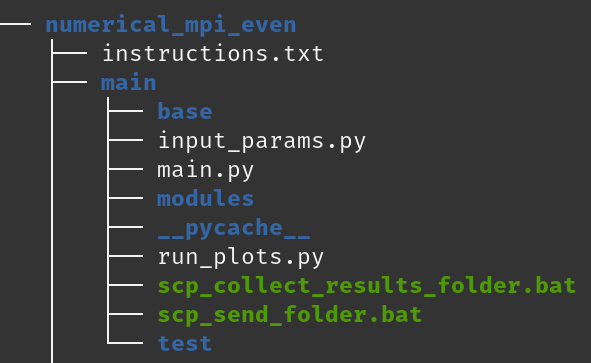
\includegraphics[width=0.45\textwidth]{figures/parallel_dir0.png}
    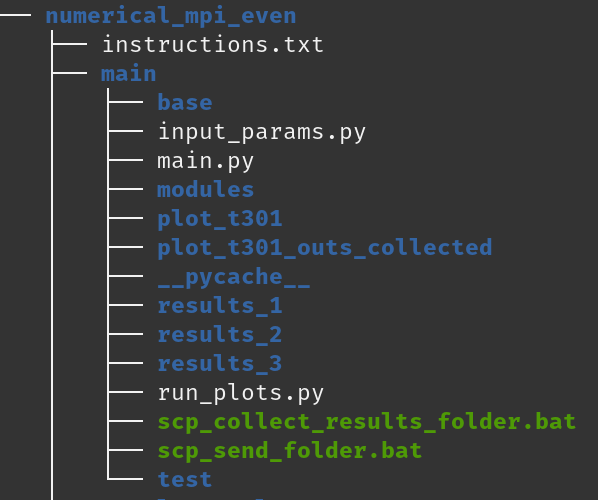
\includegraphics[width=0.45\textwidth]{figures/parallel_dir1.png}
    \caption{Contents within the directory before and after running \texttt{main.py}}
\end{figure}

The \texttt{base/} directory contains \texttt{ftcs.py} file with additional functionalities to enable parallelization. \texttt{main.py} copies the \texttt{base/} to the \texttt{results\_*/} directories, with the parameters $\tau$, $h$ and \texttt{size} initialized for each particular subcase.

\begin{figure}[H]
\begin{lstlisting}[language=Python]
copy_files_base_to_case()

node = assign_node() # assign appropriate node

modify_case_params() # modification of parameters in each case

run_case() # run case inside each case directory
\end{lstlisting}
\caption{Functions inside \texttt{main.py} to illustrate the automation}
\label{fig:mainpy}
\end{figure}

This is repeated 3 times, as indicated in \autoref{fig:inputparams}, resulting in the directories \texttt{results\_1/}, \texttt{results\_2/}, and \texttt{results\_3/}. Each \texttt{results} folder contains all simulations for a given $\tau$. These paramters can be changed from \texttt{input\_params.py}.

\begin{figure}[H]
\begin{lstlisting}[language=Python]
# USER INPUT for tau = 0.0001
tau = 0.0001
x_divs = [8, 16, 32, 64, 128, 256, 512, 576, 640, 704]
procs  = [1,2,4,8,16,32,64]
repeat = 3
delta_t = "plot_t401"
\end{lstlisting}
\caption{Snippet from \texttt{input\_params.py} showing user input}
\label{fig:inputparams}
\end{figure}

The process of submitting each case through \texttt{SLURM} is automated in \texttt{script\_main.py} found inside \texttt{modules/}, these functions are utitlized in \texttt{main.py} as shown in \autoref{fig:mainpy}. This also makes sure that the appropriate \texttt{nodes} are selected based on the amount of processors used. To avoid overloading, a new case is submitted once the previous is completed or the program at least waits a certain amount of time before submitting.

\begin{lstlisting}[language=Python]
os.system("sbatch submit_script.sh")
\end{lstlisting}

After execution, the program also prompts to run \texttt{run\_plots.py} to generate the relevant plots. This program can be run separately as well, provided the \texttt{results\_*} folders exist and the parameters provided in \texttt{input\_params.py} are not changed.
\begin{lstlisting}[language=sh]
$ python run_plots.py
\end{lstlisting}

\subsection{Scalability Plot: Strong Scaling}
Since we are already sure about the correctness of the program from \autoref{subsec:results} because we're using the same implementation of the FTCS from the serial section. Here, we will be mostly focusing on the performance of our parallelization, i.e. the time taken to execute the numerical method in relation with the amount of processes used. The plots shown in this section are the strong scaling plots and the comparion of execution times for all cases from \autoref{tab:DomainDecomposition1} and \autoref{tab:DomainDecomposition2}.

For the strong scaling, the size of the problem is kept constant, and the Speed-up$(\frac{t_n}{t_1})$ is observed in relation with the increase in the number of processes (i.e \texttt{size}). Here, the speed-up is the ratio of $t_n$ (the execution time for $n$ processes) to $t_1$ (execution time for 1 process or the serial process).

\begin{figure}[H]
    \centering
    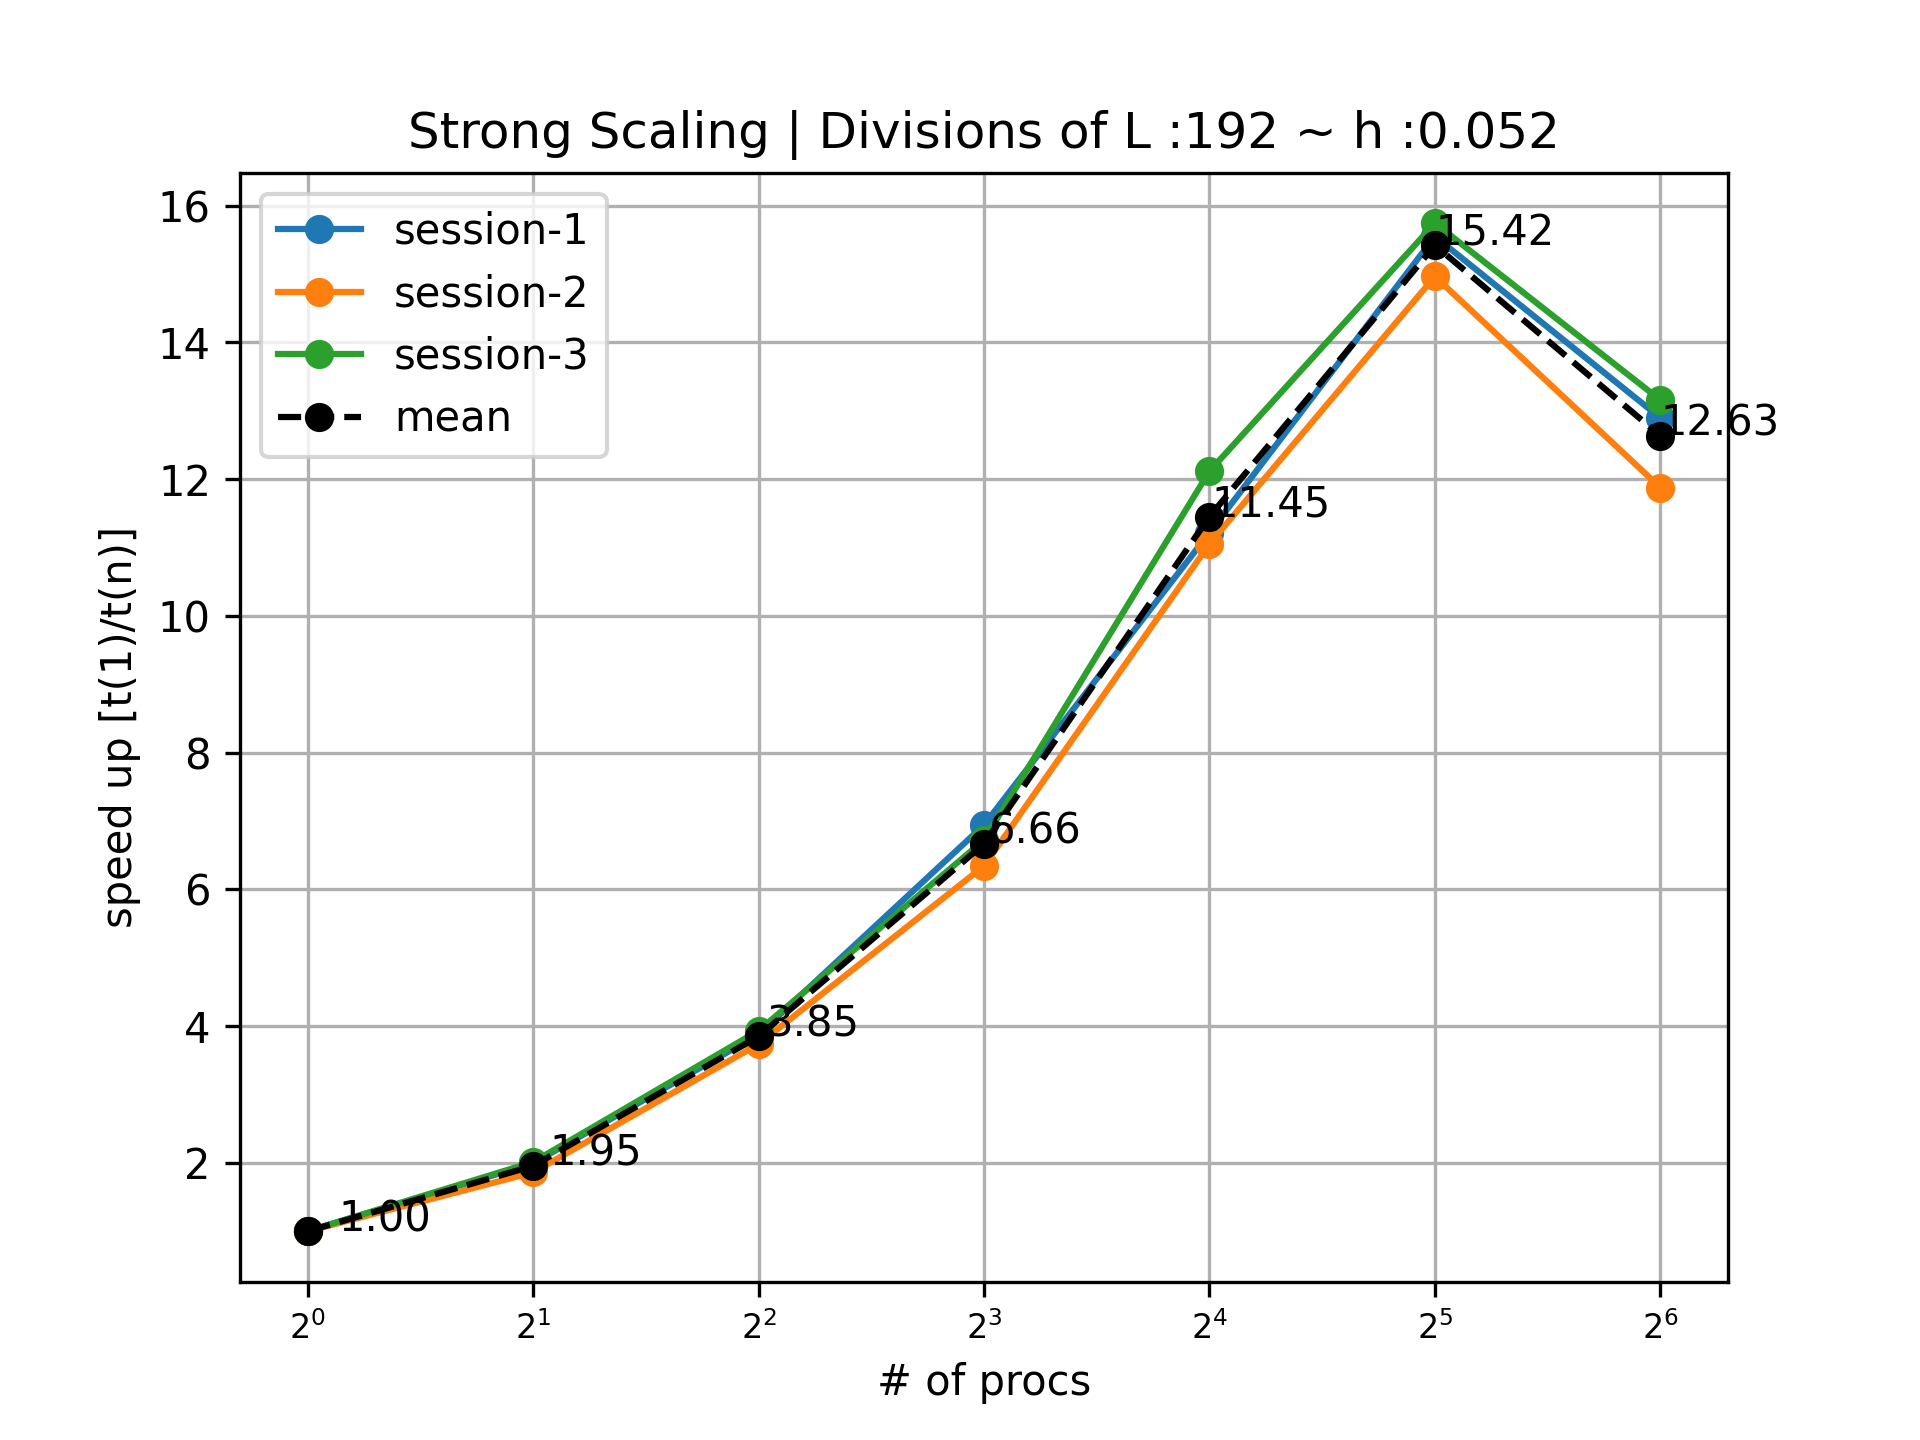
\includegraphics[width=0.7\textwidth]{figures/t301_scaling192-plot.png}
    \caption{Strong Scaling Plot for $\tau=0.001$, this shows the speed up in time with increase in \texttt{size}}
    \label{fig:t301scaling}
\end{figure}
The plots in \autoref{fig:t301scaling} and \autoref{fig:t401scaling} show the speed up in the execution time with increase in the number of processes. It can be observed that with each successive power of 2 in the number of processes, the speed-up nearly doubles from the previous step. 

The sudden decrease in speed-up at the end can be explained by the fact that the overall communication between a large a number of processes is significantly more than the local problem size within each process. Thus, regardless of the speed of the numerical method, the high communication overhead between processes slows down the overall performance.

\begin{figure}[H]
    \centering
    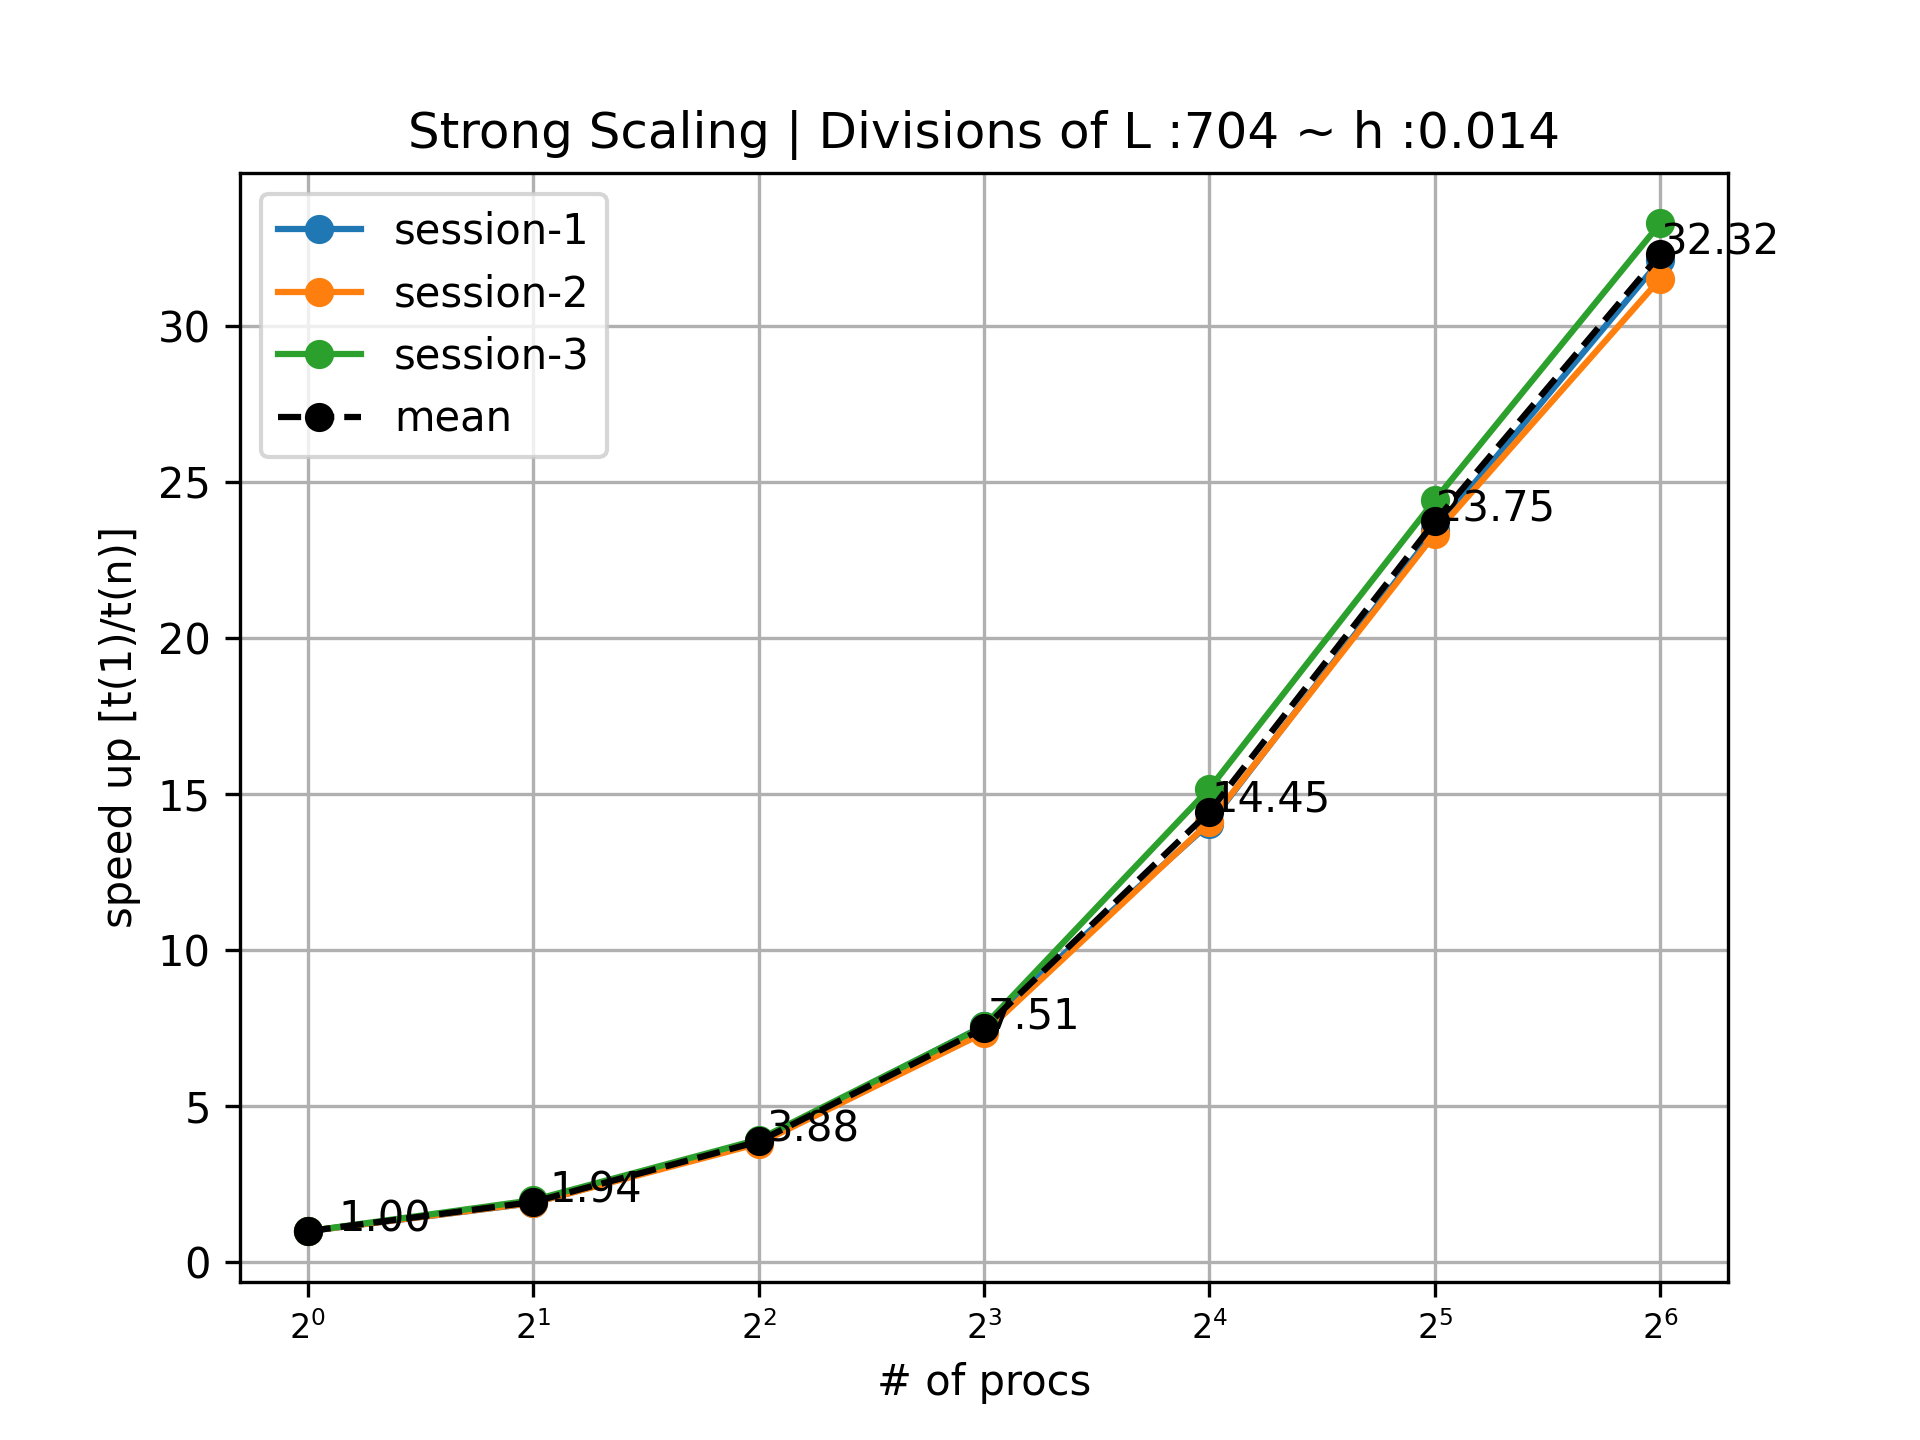
\includegraphics[width=0.7\textwidth]{figures/t401_scaling704-plot.png}
    \caption{Strong Scaling Plot for $\tau=0.0001$, this shows the speed up in time with increase in \texttt{size}}
    \label{fig:t401scaling}
\end{figure}


\begin{figure}[H]
    \centering
    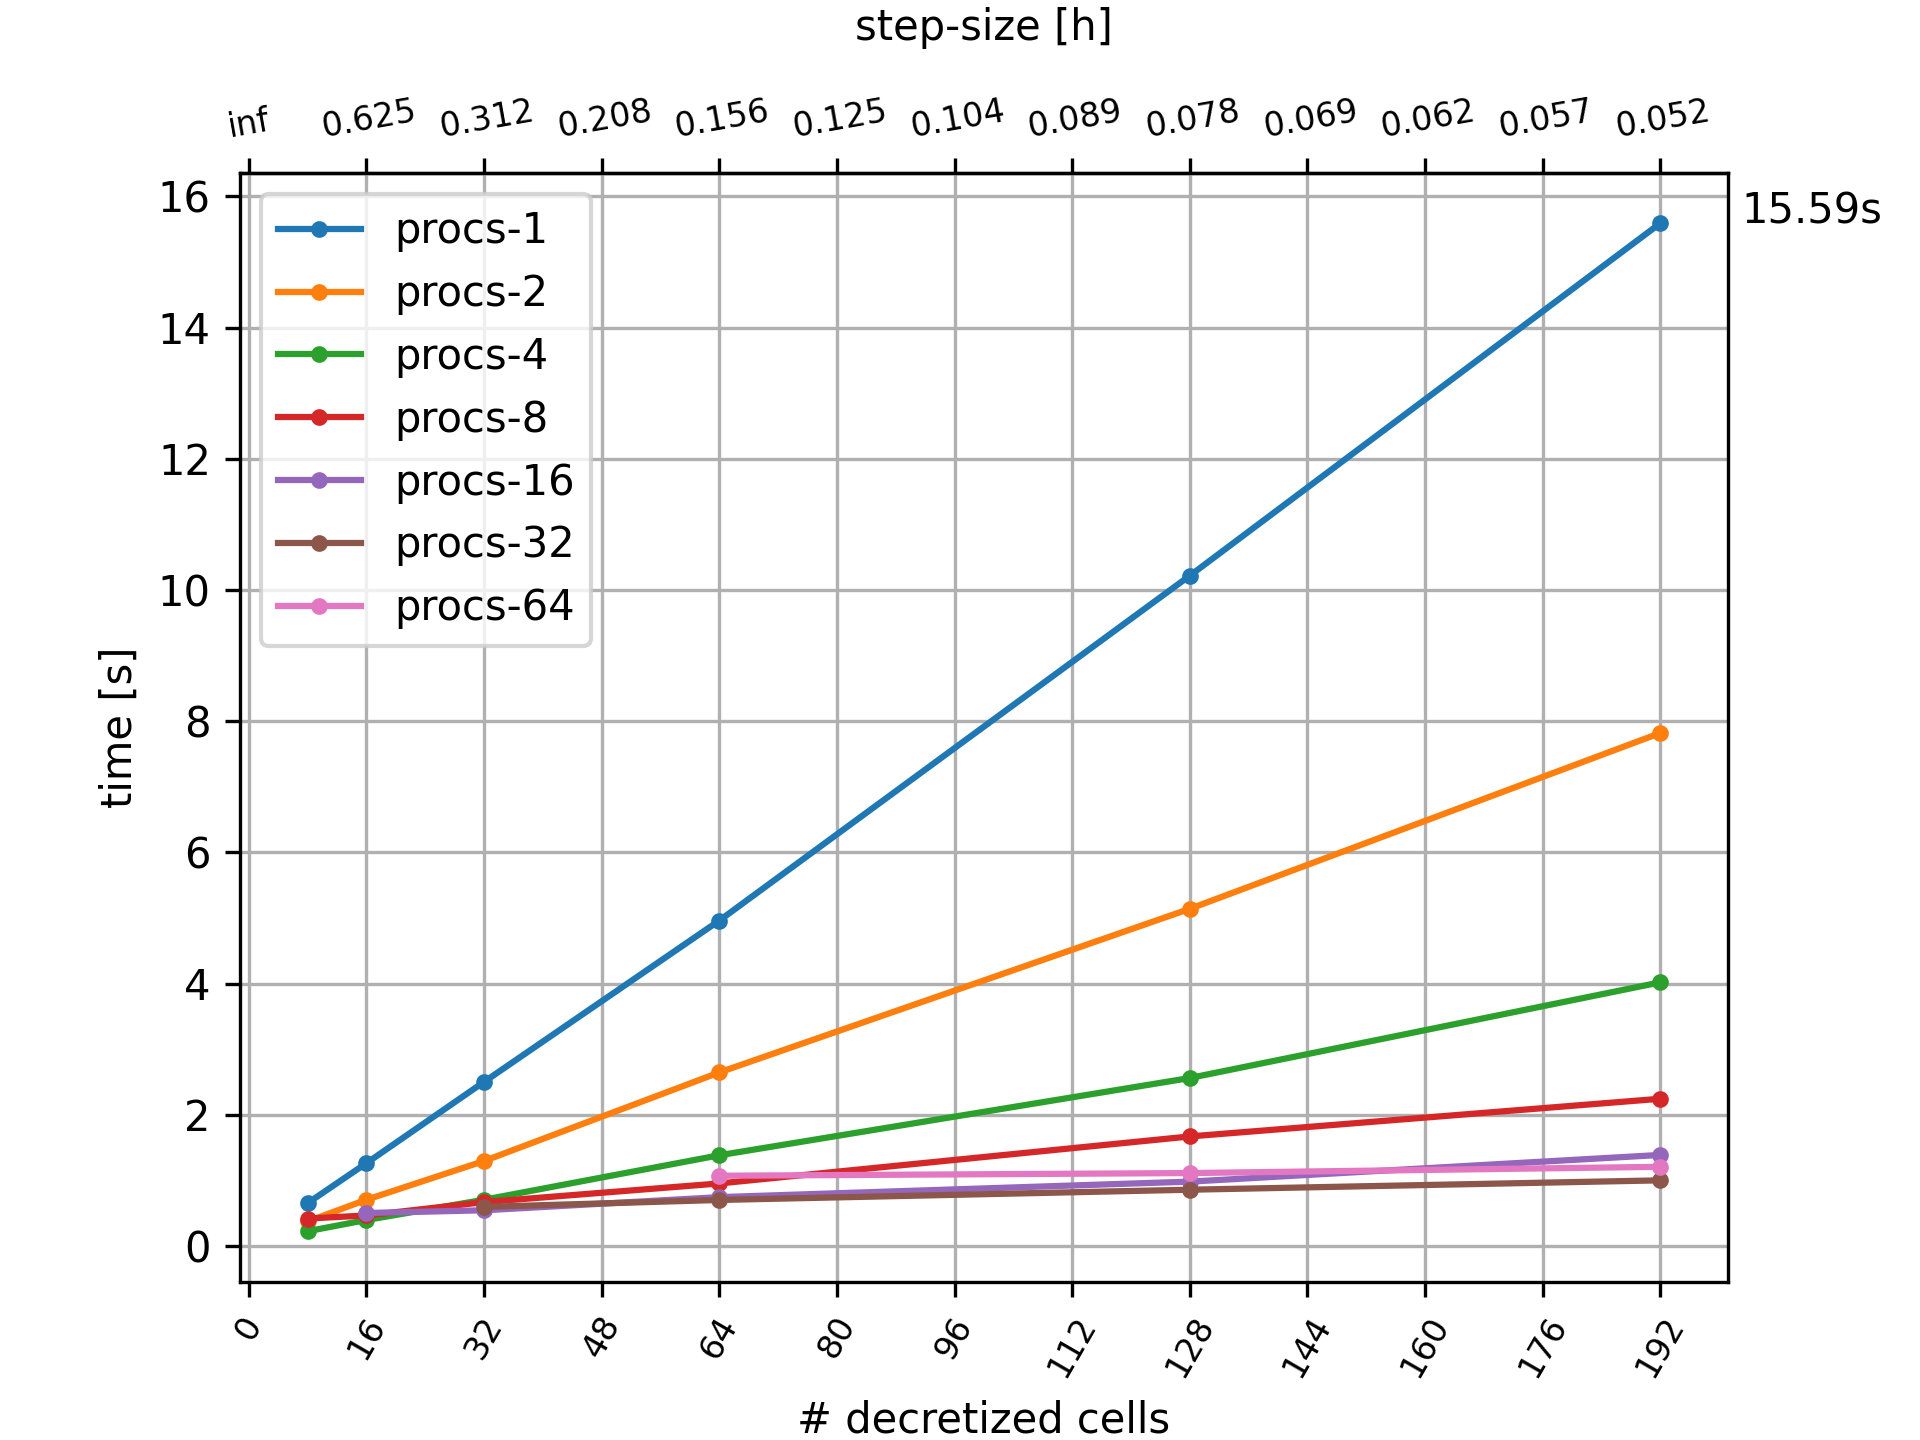
\includegraphics[width=0.7\textwidth]{figures/t301_const_proc_plot.png}
    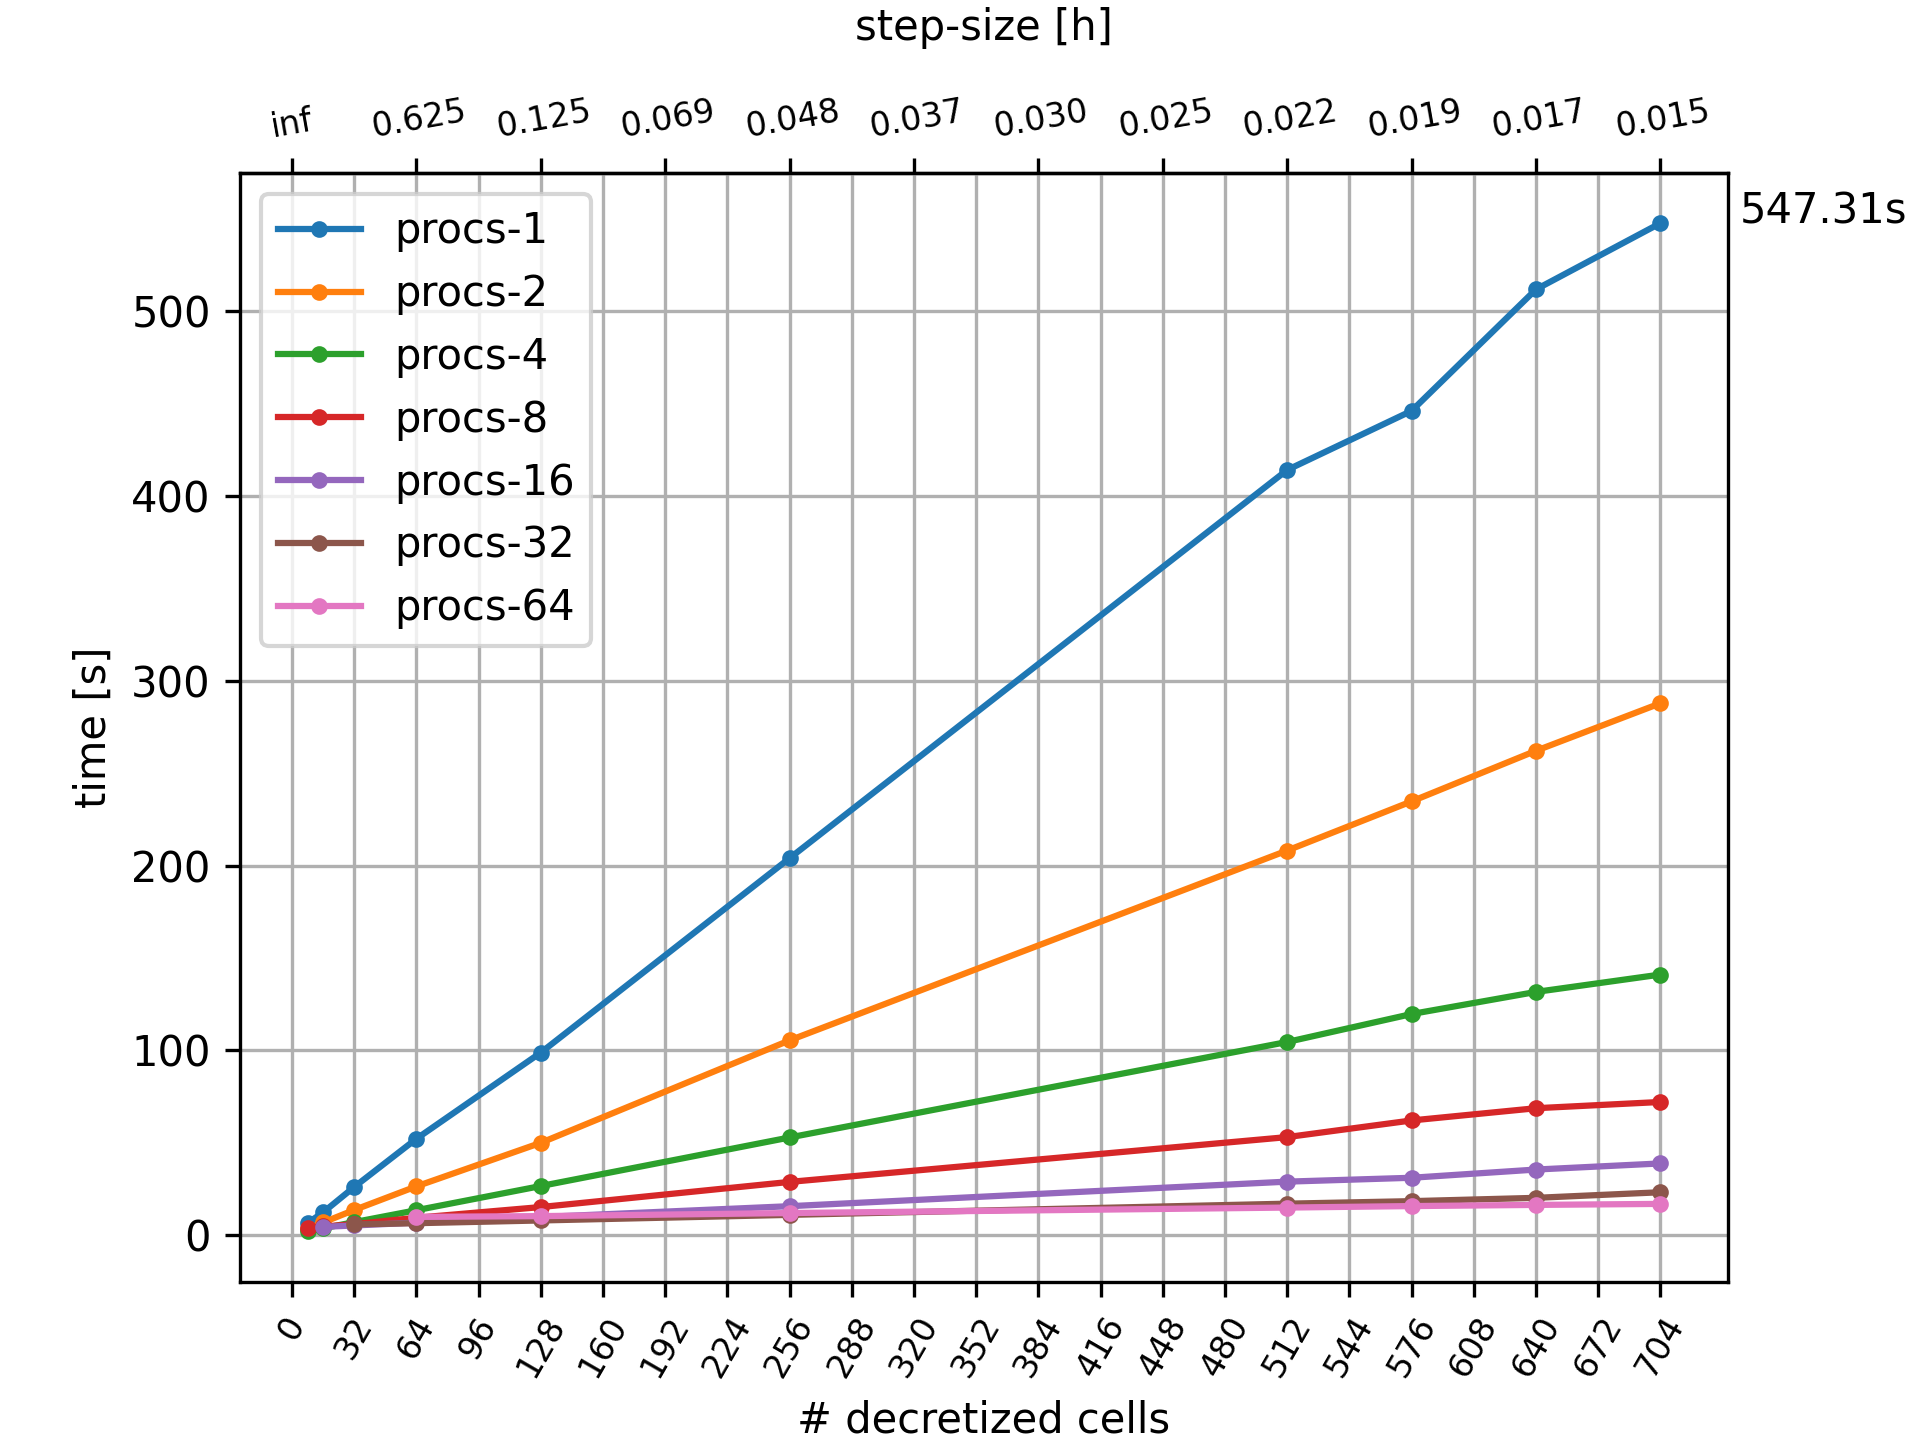
\includegraphics[width=0.7\textwidth, trim = 0 0 0 0.5cm, clip]{figures/t401_const_proc_plot.png}
    \caption{Execution times of all cases in \autoref{tab:DomainDecomposition1} (top) and \autoref{tab:DomainDecomposition2} (bottom)}
    \label{fig:allexec}
\end{figure}

It can be observed from \autoref{fig:allexec} that the doubling of speed-up with increase in processors (or the halving of execution times) is true for other problem sizes as well. We can also recognize the effect of communication overhead for \texttt{procs-64} in the plot at the top.